% 5chain.tex
% TikZ schematic of a regular 5-chain: five lines l_1,...,l_5 with only consecutive intersections
% Usage: % 5chain.tex
% TikZ schematic of a regular 5-chain: five lines l_1,...,l_5 with only consecutive intersections
% Usage: % 5chain.tex
% TikZ schematic of a regular 5-chain: five lines l_1,...,l_5 with only consecutive intersections
% Usage: % 5chain.tex
% TikZ schematic of a regular 5-chain: five lines l_1,...,l_5 with only consecutive intersections
% Usage: \input{figures/5chain.tex} inside a figure environment
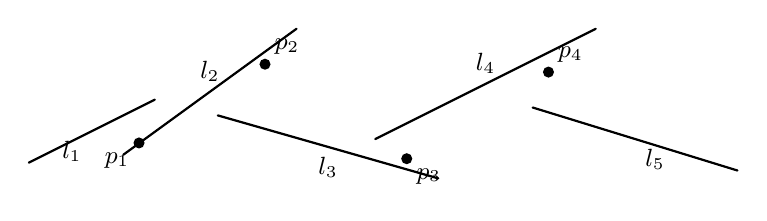
\begin{tikzpicture}[scale=1.0, every node/.style={font=\small}, line cap=round, line join=round]
  % Define intersection points (not all used directly as segment endpoints to avoid extra intersections)
  \coordinate (p1) at (0,0);
  \coordinate (p2) at (2,0.7);
  \coordinate (p3) at (4,-0.2);
  \coordinate (p4) at (6,0.6);
  % Draw five lines; extend a bit beyond intersection points to show they are lines, not just segments
  % l1 passes through p1 and toward p2
  \draw[line width=0.8pt] (-0.8,-0.4) -- (0.8,0.4) node[midway, below left] {$l_1$};
  % l2 meets l1 at p1? (We instead have them meet at a point close to p1 but keep clarity). Ensure intersection only with l3 at p2.
  % Simpler: enforce intersections at labeled points p1..p4 sequentially.
  % Redefine approach: we actually mark intersection dots along drawn lines; adjacency ensured by geometry.
  \draw[line width=0.8pt] (0.4,-0.3) -- (2.6,1.3) node[midway, above] {$l_2$};
  \draw[line width=0.8pt] (1.6,0.2) -- (4.4,-0.6) node[midway, below] {$l_3$};
  \draw[line width=0.8pt] (3.6,-0.1) -- (6.4,1.3) node[midway, above] {$l_4$};
  \draw[line width=0.8pt] (5.6,0.3) -- (8.2,-0.5) node[midway, below right] {$l_5$};
  % Intersection points (visual placements chosen to lie on successive line pairs only)
  \fill (0.6,-0.15) circle (2pt) node[below left] {$p_1$};
  \fill (2.2,0.85) circle (2pt) node[above right] {$p_2$};
  \fill (4.0,-0.35) circle (2pt) node[below right] {$p_3$};
  \fill (5.8,0.75) circle (2pt) node[above right] {$p_4$};
\end{tikzpicture}
 inside a figure environment
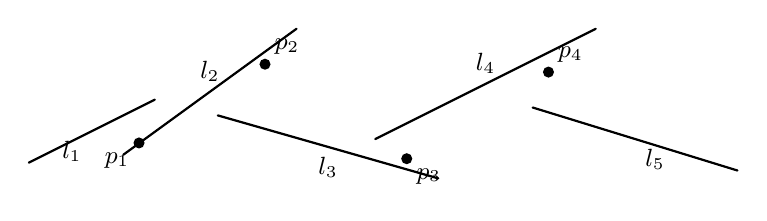
\begin{tikzpicture}[scale=1.0, every node/.style={font=\small}, line cap=round, line join=round]
  % Define intersection points (not all used directly as segment endpoints to avoid extra intersections)
  \coordinate (p1) at (0,0);
  \coordinate (p2) at (2,0.7);
  \coordinate (p3) at (4,-0.2);
  \coordinate (p4) at (6,0.6);
  % Draw five lines; extend a bit beyond intersection points to show they are lines, not just segments
  % l1 passes through p1 and toward p2
  \draw[line width=0.8pt] (-0.8,-0.4) -- (0.8,0.4) node[midway, below left] {$l_1$};
  % l2 meets l1 at p1? (We instead have them meet at a point close to p1 but keep clarity). Ensure intersection only with l3 at p2.
  % Simpler: enforce intersections at labeled points p1..p4 sequentially.
  % Redefine approach: we actually mark intersection dots along drawn lines; adjacency ensured by geometry.
  \draw[line width=0.8pt] (0.4,-0.3) -- (2.6,1.3) node[midway, above] {$l_2$};
  \draw[line width=0.8pt] (1.6,0.2) -- (4.4,-0.6) node[midway, below] {$l_3$};
  \draw[line width=0.8pt] (3.6,-0.1) -- (6.4,1.3) node[midway, above] {$l_4$};
  \draw[line width=0.8pt] (5.6,0.3) -- (8.2,-0.5) node[midway, below right] {$l_5$};
  % Intersection points (visual placements chosen to lie on successive line pairs only)
  \fill (0.6,-0.15) circle (2pt) node[below left] {$p_1$};
  \fill (2.2,0.85) circle (2pt) node[above right] {$p_2$};
  \fill (4.0,-0.35) circle (2pt) node[below right] {$p_3$};
  \fill (5.8,0.75) circle (2pt) node[above right] {$p_4$};
\end{tikzpicture}
 inside a figure environment
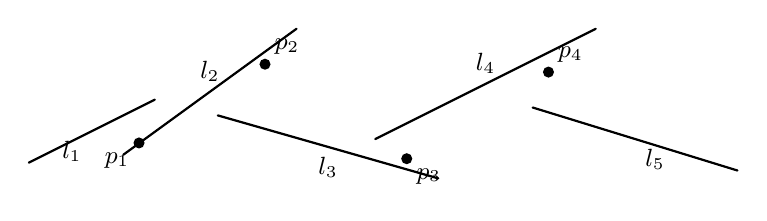
\begin{tikzpicture}[scale=1.0, every node/.style={font=\small}, line cap=round, line join=round]
  % Define intersection points (not all used directly as segment endpoints to avoid extra intersections)
  \coordinate (p1) at (0,0);
  \coordinate (p2) at (2,0.7);
  \coordinate (p3) at (4,-0.2);
  \coordinate (p4) at (6,0.6);
  % Draw five lines; extend a bit beyond intersection points to show they are lines, not just segments
  % l1 passes through p1 and toward p2
  \draw[line width=0.8pt] (-0.8,-0.4) -- (0.8,0.4) node[midway, below left] {$l_1$};
  % l2 meets l1 at p1? (We instead have them meet at a point close to p1 but keep clarity). Ensure intersection only with l3 at p2.
  % Simpler: enforce intersections at labeled points p1..p4 sequentially.
  % Redefine approach: we actually mark intersection dots along drawn lines; adjacency ensured by geometry.
  \draw[line width=0.8pt] (0.4,-0.3) -- (2.6,1.3) node[midway, above] {$l_2$};
  \draw[line width=0.8pt] (1.6,0.2) -- (4.4,-0.6) node[midway, below] {$l_3$};
  \draw[line width=0.8pt] (3.6,-0.1) -- (6.4,1.3) node[midway, above] {$l_4$};
  \draw[line width=0.8pt] (5.6,0.3) -- (8.2,-0.5) node[midway, below right] {$l_5$};
  % Intersection points (visual placements chosen to lie on successive line pairs only)
  \fill (0.6,-0.15) circle (2pt) node[below left] {$p_1$};
  \fill (2.2,0.85) circle (2pt) node[above right] {$p_2$};
  \fill (4.0,-0.35) circle (2pt) node[below right] {$p_3$};
  \fill (5.8,0.75) circle (2pt) node[above right] {$p_4$};
\end{tikzpicture}
 inside a figure environment
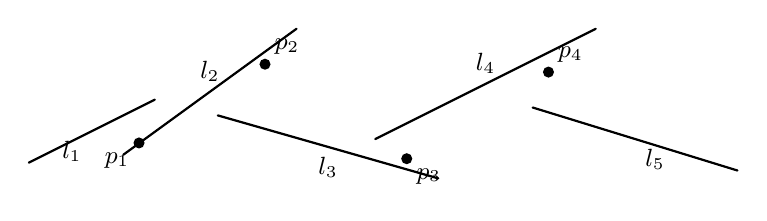
\begin{tikzpicture}[scale=1.0, every node/.style={font=\small}, line cap=round, line join=round]
  % Define intersection points (not all used directly as segment endpoints to avoid extra intersections)
  \coordinate (p1) at (0,0);
  \coordinate (p2) at (2,0.7);
  \coordinate (p3) at (4,-0.2);
  \coordinate (p4) at (6,0.6);
  % Draw five lines; extend a bit beyond intersection points to show they are lines, not just segments
  % l1 passes through p1 and toward p2
  \draw[line width=0.8pt] (-0.8,-0.4) -- (0.8,0.4) node[midway, below left] {$l_1$};
  % l2 meets l1 at p1? (We instead have them meet at a point close to p1 but keep clarity). Ensure intersection only with l3 at p2.
  % Simpler: enforce intersections at labeled points p1..p4 sequentially.
  % Redefine approach: we actually mark intersection dots along drawn lines; adjacency ensured by geometry.
  \draw[line width=0.8pt] (0.4,-0.3) -- (2.6,1.3) node[midway, above] {$l_2$};
  \draw[line width=0.8pt] (1.6,0.2) -- (4.4,-0.6) node[midway, below] {$l_3$};
  \draw[line width=0.8pt] (3.6,-0.1) -- (6.4,1.3) node[midway, above] {$l_4$};
  \draw[line width=0.8pt] (5.6,0.3) -- (8.2,-0.5) node[midway, below right] {$l_5$};
  % Intersection points (visual placements chosen to lie on successive line pairs only)
  \fill (0.6,-0.15) circle (2pt) node[below left] {$p_1$};
  \fill (2.2,0.85) circle (2pt) node[above right] {$p_2$};
  \fill (4.0,-0.35) circle (2pt) node[below right] {$p_3$};
  \fill (5.8,0.75) circle (2pt) node[above right] {$p_4$};
\end{tikzpicture}
